\documentclass[tikz,margin=2mm]{standalone}
\usepackage{tikz}
\tikzset{
  hole/.style = {fill = #1, circle, minimum width = 2.5mm, inner sep = 0mm},
  wire/.style = {draw = #1, line width = .5mm},
  label/.style = {rotate = #1, black!50!white, anchor = center},
}
\begin{document}
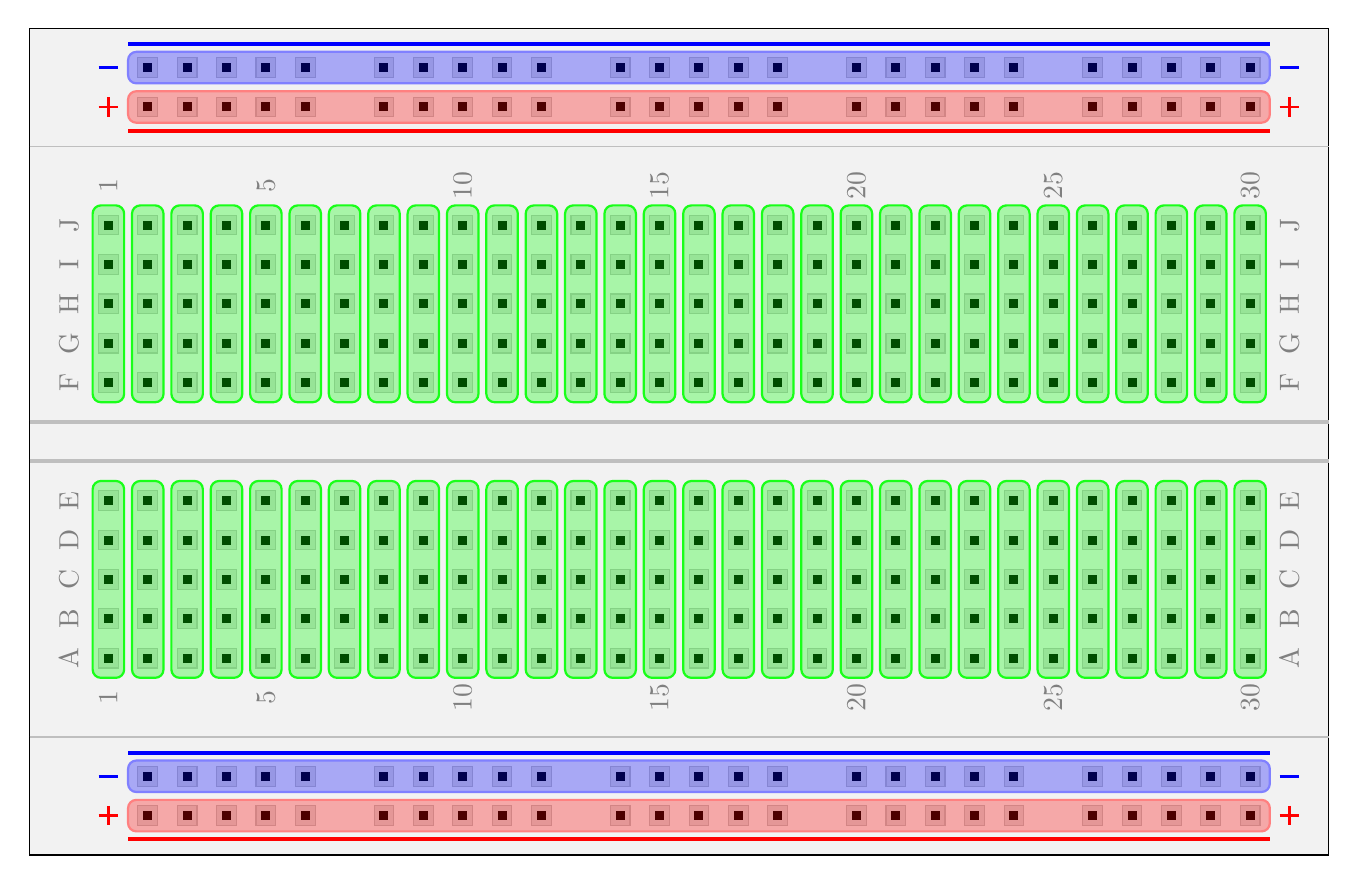
\begin{tikzpicture}[x=5mm,y=5mm]
  \draw[fill=black!05!white] (-1,-4) rectangle (32,17);
  \draw[wire=red]  (1.5,-3.6) -- (30.5,-3.6);
  \draw[wire=blue] (1.5,-1.4) -- (30.5,-1.4);
  \draw[wire=red]  (1.5,14.4) -- (30.5,14.4);
  \draw[wire=blue] (1.5,16.6) -- (30.5,16.6);
  \draw[wire=gray!50] (-1,6) -- (32,6);
  \draw[wire=gray!50] (-1,7) -- (32,7);
  \draw[wire=gray!50, line width = 0.5] (-1,14) -- (32,14);
  \draw[wire=gray!50, line width = 0.5] (-1,-1) -- (32,-1);

  \draw[blue, line width=1](0.75,-2) -- (1.25,-2);
  \draw[red, line width=1](0.75,-3) -- (1.25,-3);
  \draw[red, line width=1](1,-2.75) -- (1,-3.25);
  \draw[blue, line width=1](0.75,16) -- (1.25,16);
  \draw[red, line width=1](0.75,15) -- (1.25,15);
  \draw[red, line width=1](1,14.75) -- (1,15.25);
  
  \draw[blue, line width=1](30.75,-2) -- (31.25,-2);
  \draw[red, line width=1](30.75,-3) -- (31.25,-3);
  \draw[red, line width=1](31,-2.75) -- (31,-3.25);
  \draw[blue, line width=1](30.75,16) -- (31.25,16);
  \draw[red, line width=1](30.75,15) -- (31.25,15);
  \draw[red, line width=1](31,14.75) -- (31,15.25);
 
  \foreach \xi in {2,...,6,8,9,...,12,14,15,...,18,20,21,...,24,26,27,...,30} {
  	\draw[draw=gray!50, fill=gray!30] (\xi+0.25,-1.75) rectangle ++(-0.5, -0.5);
  	\draw[fill=black] (\xi+0.1,-2+0.1) rectangle ++(-0.2, -0.2);
  	\draw[draw=gray!50, fill=gray!30] (\xi+0.25,-2.75) rectangle ++(-0.5, -0.5);
  	\draw[fill=black] (\xi+0.1,-3+0.1) rectangle ++(-0.2, -0.2);
  	\draw[draw=gray!50, fill=gray!30] (\xi+0.25,15.25) rectangle ++(-0.5, -0.5);
  	\draw[fill=black] (\xi+0.1,15+0.1) rectangle ++(-0.2, -0.2);
  	\draw[draw=gray!50, fill=gray!30] (\xi+0.25,16.25) rectangle ++(-0.5, -0.5);
  	\draw[fill=black] (\xi+0.1,16+0.1) rectangle ++(-0.2, -0.2);
  }
  
  \foreach \xi in {1,...,30}{
    \foreach \ys in {0,7}{
      \foreach \yi in {1,2,3,4,5}{
        \draw[draw=gray!50, fill=gray!30] (\xi+0.25,\yi+\ys+0.25) rectangle ++(-0.5, -0.5);
        \draw[fill=black] (\xi+0.10,\yi+\ys-0.10) rectangle ++(-0.2, 0.2);
      }
    }
  }
  \foreach \m/\yi in {A/1,B/2,C/3,D/4,E/5,F/8,G/9,H/10,I/11,J/12}{
    \node[label=90] at ( 0,\yi) {\m};
    \node[label=90] at (31,\yi) {\m};
  }
  \foreach \m/\xi in {1,5,10,...,30}{
    \node[label=90] at (\xi, 0) {\m};
    \node[label=90] at (\xi,13) {\m};
  }
  
  \foreach \xi in {0,...,29}{
    \draw[rounded corners=3pt, thick, draw=green!90, fill=green, fill opacity=0.3] (\xi+0.6,7.5) rectangle (\xi+1.4,12.5);
    \draw[rounded corners=3pt, thick, draw=green!90, fill=green, fill opacity=0.3] (\xi+0.6,0.5) rectangle (\xi+1.4,5.5);
  }
  
  \draw[rounded corners=3pt, thick, draw=blue!50, fill=blue, fill opacity=0.3] (1.5,15.6) rectangle (30.5,16.4);
  \draw[rounded corners=3pt, thick, draw=red!50, fill=red, fill opacity=0.3] (1.5,14.6) rectangle (30.5,15.4);
  
  \draw[rounded corners=3pt, thick, draw=red!50, fill=red, fill opacity=0.3] (1.5,-3.4) rectangle (30.5,-2.6);
  \draw[rounded corners=3pt, thick, draw=blue!50, fill=blue, fill opacity=0.3] (1.5,-2.4) rectangle (30.5,-1.6);
\end{tikzpicture}
\end{document}